% Options for packages loaded elsewhere
% Options for packages loaded elsewhere
\PassOptionsToPackage{unicode}{hyperref}
\PassOptionsToPackage{hyphens}{url}
%
\documentclass[
  ignorenonframetext,
  aspectratio=169,
  russian,
]{beamer}
\newif\ifbibliography
\usepackage{pgfpages}
\setbeamertemplate{caption}[numbered]
\setbeamertemplate{caption label separator}{: }
\setbeamercolor{caption name}{fg=normal text.fg}
\beamertemplatenavigationsymbolshorizontal
% Prevent slide breaks in the middle of a paragraph
\widowpenalties 1 10000
\raggedbottom
\AtBeginPart{
  \frame{\partpage}
}
\AtBeginSection{
  \ifbibliography
  \else
    \frame{\sectionpage}
  \fi
}
\AtBeginSubsection{
  \frame{\subsectionpage}
}
\usepackage{iftex}
\ifPDFTeX
  \usepackage[T1]{fontenc}
  \usepackage[utf8]{inputenc}
  \usepackage{textcomp} % provide euro and other symbols
\else % if luatex or xetex
  \usepackage{unicode-math} % this also loads fontspec
  \defaultfontfeatures{Scale=MatchLowercase}
  \defaultfontfeatures[\rmfamily]{Ligatures=TeX,Scale=1}
\fi
\usepackage{lmodern}

\usetheme[]{Montpellier}
\usecolortheme[]{seagull}
\ifPDFTeX\else
  % xetex/luatex font selection
\fi
% Use upquote if available, for straight quotes in verbatim environments
\IfFileExists{upquote.sty}{\usepackage{upquote}}{}
\IfFileExists{microtype.sty}{% use microtype if available
  \usepackage[]{microtype}
  \UseMicrotypeSet[protrusion]{basicmath} % disable protrusion for tt fonts
}{}


\usepackage{longtable,booktabs,array}
\usepackage{calc} % for calculating minipage widths
\usepackage{caption}
% Make caption package work with longtable
\makeatletter
\def\fnum@table{\tablename~\thetable}
\makeatother
\usepackage{graphicx}
\makeatletter
\newsavebox\pandoc@box
\newcommand*\pandocbounded[1]{% scales image to fit in text height/width
  \sbox\pandoc@box{#1}%
  \Gscale@div\@tempa{\textheight}{\dimexpr\ht\pandoc@box+\dp\pandoc@box\relax}%
  \Gscale@div\@tempb{\linewidth}{\wd\pandoc@box}%
  \ifdim\@tempb\p@<\@tempa\p@\let\@tempa\@tempb\fi% select the smaller of both
  \ifdim\@tempa\p@<\p@\scalebox{\@tempa}{\usebox\pandoc@box}%
  \else\usebox{\pandoc@box}%
  \fi%
}
% Set default figure placement to htbp
\def\fps@figure{htbp}
\makeatother



\ifLuaTeX
\usepackage[bidi=basic,provide=*]{babel}
\else
\usepackage[bidi=default,provide=*]{babel}
\fi
% get rid of language-specific shorthands (see #6817):
\let\LanguageShortHands\languageshorthands
\def\languageshorthands#1{}


\setlength{\emergencystretch}{3em} % prevent overfull lines

\providecommand{\tightlist}{%
  \setlength{\itemsep}{0pt}\setlength{\parskip}{0pt}}



 

\usepackage[]{csquotes}

\usepackage{libertine}
\makeatletter
\@ifpackageloaded{caption}{}{\usepackage{caption}}
\AtBeginDocument{%
\ifdefined\contentsname
  \renewcommand*\contentsname{Содержание}
\else
  \newcommand\contentsname{Содержание}
\fi
\ifdefined\listfigurename
  \renewcommand*\listfigurename{Список иллюстраций}
\else
  \newcommand\listfigurename{Список иллюстраций}
\fi
\ifdefined\listtablename
  \renewcommand*\listtablename{Список таблиц}
\else
  \newcommand\listtablename{Список таблиц}
\fi
\ifdefined\figurename
  \renewcommand*\figurename{Рисунок}
\else
  \newcommand\figurename{Рисунок}
\fi
\ifdefined\tablename
  \renewcommand*\tablename{Таблица}
\else
  \newcommand\tablename{Таблица}
\fi
}
\@ifpackageloaded{float}{}{\usepackage{float}}
\floatstyle{ruled}
\@ifundefined{c@chapter}{\newfloat{codelisting}{h}{lop}}{\newfloat{codelisting}{h}{lop}[chapter]}
\floatname{codelisting}{Список}
\newcommand*\listoflistings{\listof{codelisting}{Листинги}}
\makeatother
\makeatletter
\makeatother
\makeatletter
\@ifpackageloaded{caption}{}{\usepackage{caption}}
\@ifpackageloaded{subcaption}{}{\usepackage{subcaption}}
\makeatother

\usepackage{bookmark}
\IfFileExists{xurl.sty}{\usepackage{xurl}}{} % add URL line breaks if available
\urlstyle{same}
\hypersetup{
  pdftitle={Лабораторная работа №7},
  pdfauthor={Поляков Глеб Сергеевич},
  pdflang={ru-RU},
  hidelinks,
  pdfcreator={LaTeX via pandoc}}


\title{Лабораторная работа №7}
\subtitle{Компьютерный практикум по статистическому анализу данных}
\author{Поляков Глеб Сергеевич}
\date{2025-12-06}

\begin{document}
\frame{\titlepage}

\renewcommand*\contentsname{Содержание}
\begin{frame}[allowframebreaks]
  \frametitle{Содержание}
  \setcounter{tocdepth}{2}
  \tableofcontents
\end{frame}
\setcounter{tocdepth}{2}
\tableofcontents
}

\section{1. Информация}\label{ux438ux43dux444ux43eux440ux43cux430ux446ux438ux44f}

\begin{frame}{1.1 Докладчик}
\phantomsection\label{ux434ux43eux43aux43bux430ux434ux447ux438ux43a}
\begin{columns}[c]
\begin{column}{0.7\linewidth}
\begin{itemize}[<+->]
\tightlist
\item
  Поляков Глеб Сергеевич
\item
  Студент
\item
  Российский университет дружбы народов им. П. Лумумбы
\end{itemize}
\end{column}

\begin{column}{0.3\linewidth}
\begin{frame}{1.2 Цель лабораторной работы}
\phantomsection\label{ux446ux435ux43bux44c-ux43bux430ux431ux43eux440ux430ux442ux43eux440ux43dux43eux439-ux440ux430ux431ux43eux442ux44b}
\begin{itemize}[<+->]
\tightlist
\item
  Изучить специализированные пакеты Julia для обработки данных.
\end{itemize}
\end{frame}

\section{2. Выполнение лабораторной
работы}\label{ux432ux44bux43fux43eux43bux43dux435ux43dux438ux435-ux43bux430ux431ux43eux440ux430ux442ux43eux440ux43dux43eux439-ux440ux430ux431ux43eux442ux44b}

\begin{frame}{2.1 Julia для науки о данных}
\phantomsection\label{julia-ux434ux43bux44f-ux43dux430ux443ux43aux438-ux43e-ux434ux430ux43dux43dux44bux445}
В Julia для обработки данных используются наработки из других языков
программирования, в частности, из R и Python.
\end{frame}

\begin{frame}{2.2 Считывание данных}
\phantomsection\label{ux441ux447ux438ux442ux44bux432ux430ux43dux438ux435-ux434ux430ux43dux43dux44bux445}
\begin{figure}

{\centering 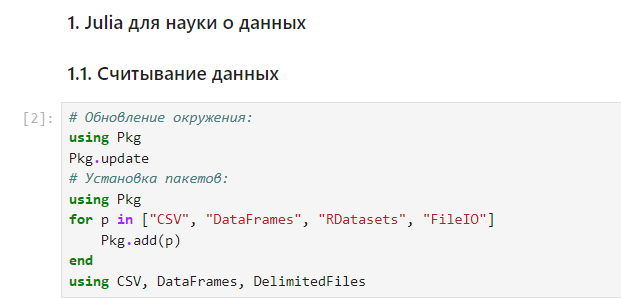
\includegraphics[width=0.8\linewidth,height=0.8\textheight]{image/1.PNG}

}

\caption{Установка пакетов}

\end{figure}%
\end{frame}

\begin{frame}{2.3 Считывание данных}
\phantomsection\label{ux441ux447ux438ux442ux44bux432ux430ux43dux438ux435-ux434ux430ux43dux43dux44bux445-1}
\begin{figure}

{\centering 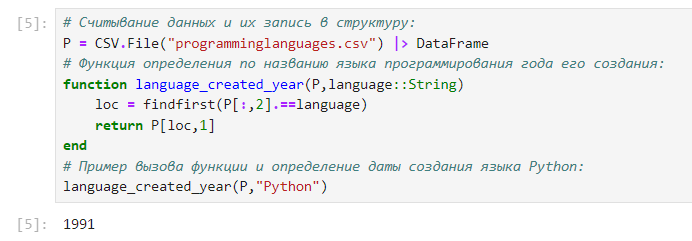
\includegraphics[width=1\linewidth,height=1\textheight]{image/2.PNG}

}

\caption{Считывание данных и запись в структуру}

\end{figure}%
\end{frame}

\begin{frame}{2.4 Считывание данных}
\phantomsection\label{ux441ux447ux438ux442ux44bux432ux430ux43dux438ux435-ux434ux430ux43dux43dux44bux445-2}
\begin{figure}

{\centering 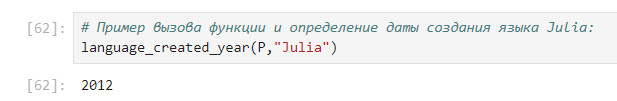
\includegraphics[width=1\linewidth,height=1\textheight]{image/3.PNG}

}

\caption{Пример}

\end{figure}%
\end{frame}

\begin{frame}{2.5 Считывание данных}
\phantomsection\label{ux441ux447ux438ux442ux44bux432ux430ux43dux438ux435-ux434ux430ux43dux43dux44bux445-3}
\begin{figure}

{\centering 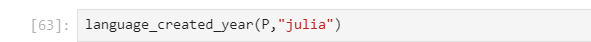
\includegraphics[width=1\linewidth,height=1\textheight]{image/4.PNG}

}

\caption{Поиск \enquote{julia} со строчной буквы}

\end{figure}%
\end{frame}

\begin{frame}{2.6 Считывание данных}
\phantomsection\label{ux441ux447ux438ux442ux44bux432ux430ux43dux438ux435-ux434ux430ux43dux43dux44bux445-4}
\begin{figure}

{\centering 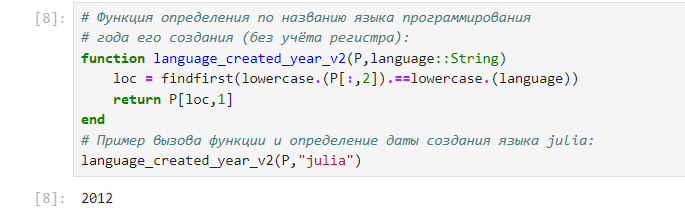
\includegraphics[width=1\linewidth,height=1\textheight]{image/5.PNG}

}

\caption{Изменение исходной функции}

\end{figure}%
\end{frame}

\begin{frame}{2.7 Считывание данных}
\phantomsection\label{ux441ux447ux438ux442ux44bux432ux430ux43dux438ux435-ux434ux430ux43dux43dux44bux445-5}
\begin{figure}

{\centering 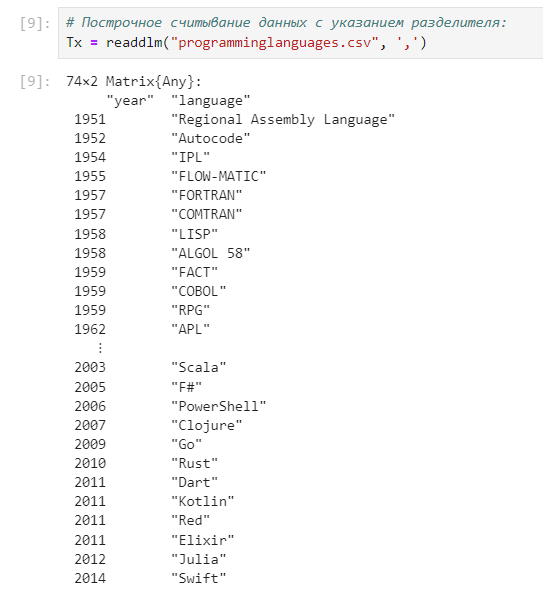
\includegraphics[width=0.8\linewidth,height=0.8\textheight]{image/6.PNG}

}

\caption{Построчное считывание данных}

\end{figure}%
\end{frame}

\begin{frame}{2.8 Запись данных в файл}
\phantomsection\label{ux437ux430ux43fux438ux441ux44c-ux434ux430ux43dux43dux44bux445-ux432-ux444ux430ux439ux43b}
\begin{figure}

{\centering 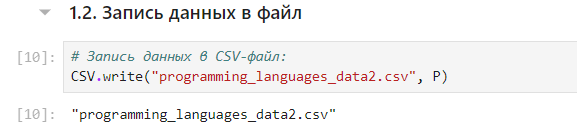
\includegraphics[width=1\linewidth,height=1\textheight]{image/7.PNG}

}

\caption{Запись данных в файл}

\end{figure}%
\end{frame}

\begin{frame}{2.9 Запись данных в файл}
\phantomsection\label{ux437ux430ux43fux438ux441ux44c-ux434ux430ux43dux43dux44bux445-ux432-ux444ux430ux439ux43b-1}
\begin{figure}

{\centering 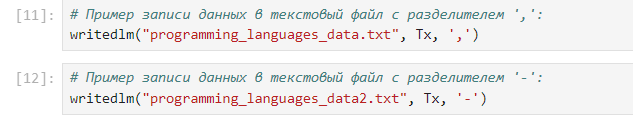
\includegraphics[width=1\linewidth,height=1\textheight]{image/8.PNG}

}

\caption{Пример с указанием типа данных и разделителем данных}

\end{figure}%
\end{frame}

\begin{frame}{2.10 Запись данных в файл}
\phantomsection\label{ux437ux430ux43fux438ux441ux44c-ux434ux430ux43dux43dux44bux445-ux432-ux444ux430ux439ux43b-2}
\begin{figure}

{\centering 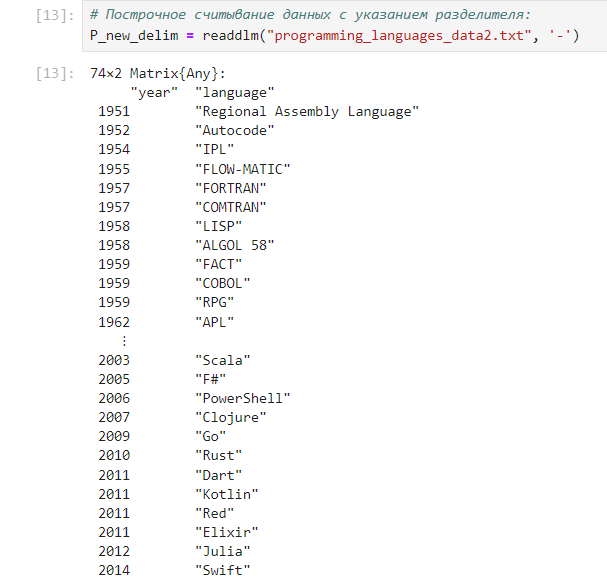
\includegraphics[width=0.8\linewidth,height=0.8\textheight]{image/9.PNG}

}

\caption{Проверка корректности считывания созданного текстового файла}

\end{figure}%
\end{frame}

\begin{frame}{2.11 Словари}
\phantomsection\label{ux441ux43bux43eux432ux430ux440ux438}
\begin{figure}

{\centering 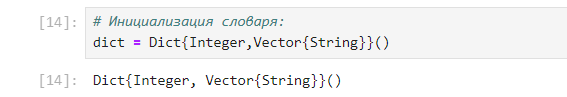
\includegraphics[width=1\linewidth,height=1\textheight]{image/10.PNG}

}

\caption{Инициализация словаря}

\end{figure}%
\end{frame}

\begin{frame}{2.12 Словари}
\phantomsection\label{ux441ux43bux43eux432ux430ux440ux438-1}
\begin{figure}

{\centering 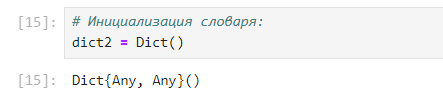
\includegraphics[width=1\linewidth,height=1\textheight]{image/11.PNG}

}

\caption{Инициализация пустого словаря}

\end{figure}%
\end{frame}

\begin{frame}{2.13 Словари}
\phantomsection\label{ux441ux43bux43eux432ux430ux440ux438-2}
\begin{figure}

{\centering 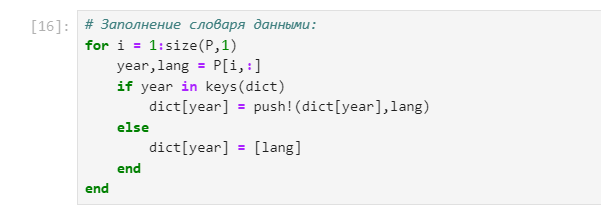
\includegraphics[width=1\linewidth,height=1\textheight]{image/12.PNG}

}

\caption{Заполнение словаря данными}

\end{figure}%
\end{frame}

\begin{frame}{2.14 Словари}
\phantomsection\label{ux441ux43bux43eux432ux430ux440ux438-3}
\begin{figure}

{\centering 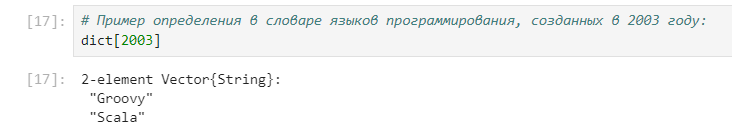
\includegraphics[width=1\linewidth,height=1\textheight]{image/13.PNG}

}

\caption{Пример работы словаря}

\end{figure}%
\end{frame}

\begin{frame}{2.15 DataFrames}
\phantomsection\label{dataframes}
\begin{figure}

{\centering 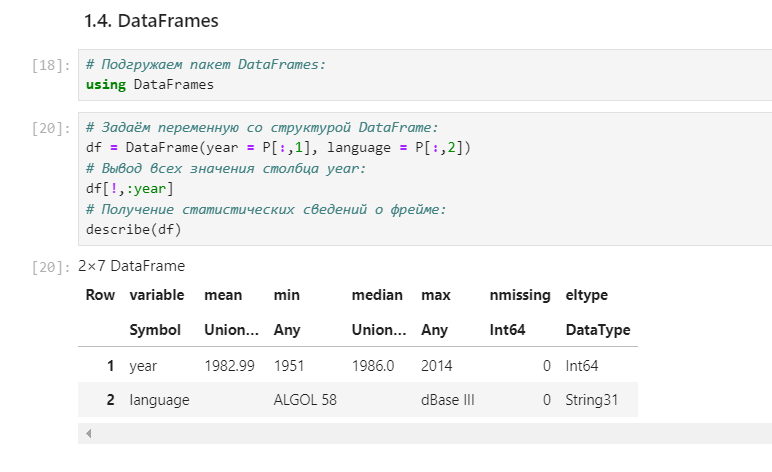
\includegraphics[width=0.8\linewidth,height=0.8\textheight]{image/14.PNG}

}

\caption{Пример создания структуры DataFrame}

\end{figure}%
\end{frame}

\begin{frame}{2.16 RDatasets}
\phantomsection\label{rdatasets}
\begin{figure}

{\centering 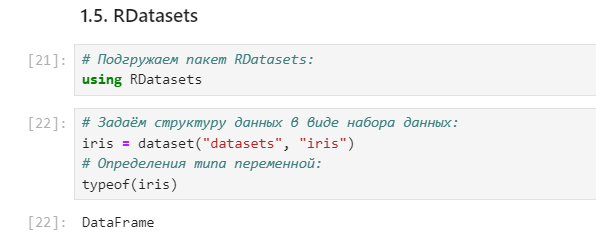
\includegraphics[width=1\linewidth,height=1\textheight]{image/15.PNG}

}

\caption{Работа с пакетом RDatasets}

\end{figure}%
\end{frame}

\begin{frame}{2.17 RDatasets}
\phantomsection\label{rdatasets-1}
\begin{figure}

{\centering 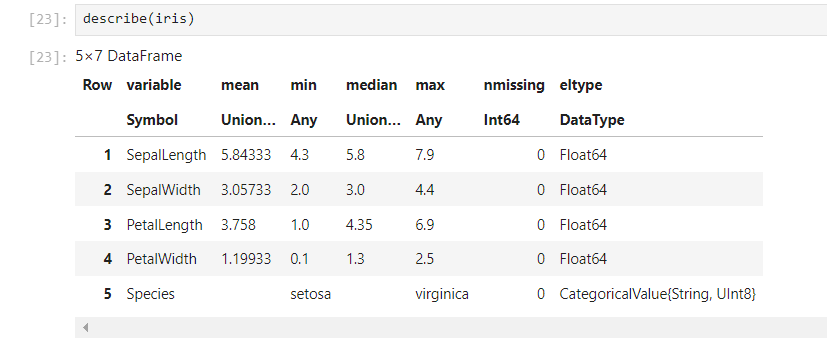
\includegraphics[width=1\linewidth,height=1\textheight]{image/16.PNG}

}

\caption{Получение основных статических сведений о каждом столбце в
наборе данных}

\end{figure}%
\end{frame}

\begin{frame}{2.18 Работа с переменными отсутствующего типа (Missing
Values)}
\phantomsection\label{ux440ux430ux431ux43eux442ux430-ux441-ux43fux435ux440ux435ux43cux435ux43dux43dux44bux43cux438-ux43eux442ux441ux443ux442ux441ux442ux432ux443ux44eux449ux435ux433ux43e-ux442ux438ux43fux430-missing-values}
\begin{figure}

{\centering 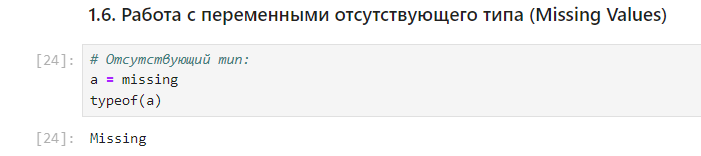
\includegraphics[width=1\linewidth,height=1\textheight]{image/17.PNG}

}

\caption{Использование \enquote{отсутствующего} типа}

\end{figure}%
\end{frame}

\begin{frame}{2.19 Работа с переменными отсутствующего типа (Missing
Values)}
\phantomsection\label{ux440ux430ux431ux43eux442ux430-ux441-ux43fux435ux440ux435ux43cux435ux43dux43dux44bux43cux438-ux43eux442ux441ux443ux442ux441ux442ux432ux443ux44eux449ux435ux433ux43e-ux442ux438ux43fux430-missing-values-1}
\begin{figure}

{\centering 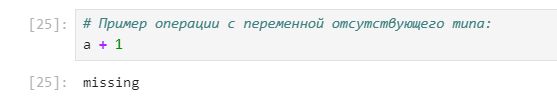
\includegraphics[width=1\linewidth,height=1\textheight]{image/18.PNG}

}

\caption{Операция сложения числа и переменной с отсутствующим типом}

\end{figure}%
\end{frame}

\begin{frame}{2.20 Работа с переменными отсутствующего типа (Missing
Values)}
\phantomsection\label{ux440ux430ux431ux43eux442ux430-ux441-ux43fux435ux440ux435ux43cux435ux43dux43dux44bux43cux438-ux43eux442ux441ux443ux442ux441ux442ux432ux443ux44eux449ux435ux433ux43e-ux442ux438ux43fux430-missing-values-2}
\begin{figure}

{\centering 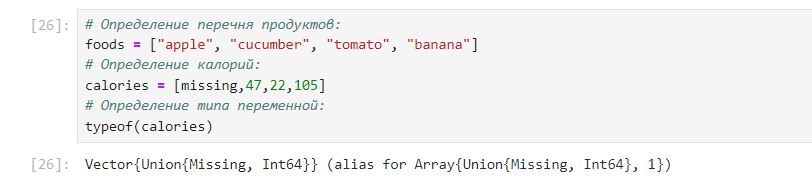
\includegraphics[width=1\linewidth,height=1\textheight]{image/19.PNG}

}

\caption{Пример работы с данными, среди которых есть данные с
отсутствующим типом}

\end{figure}%
\end{frame}

\begin{frame}{2.21 Работа с переменными отсутствующего типа (Missing
Values)}
\phantomsection\label{ux440ux430ux431ux43eux442ux430-ux441-ux43fux435ux440ux435ux43cux435ux43dux43dux44bux43cux438-ux43eux442ux441ux443ux442ux441ux442ux432ux443ux44eux449ux435ux433ux43e-ux442ux438ux43fux430-missing-values-3}
\begin{figure}

{\centering 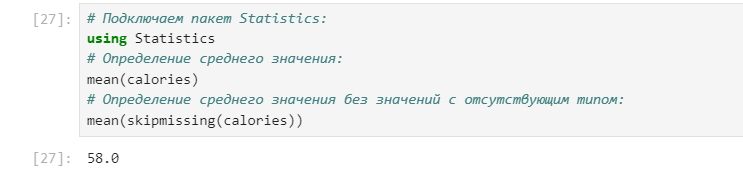
\includegraphics[width=1\linewidth,height=1\textheight]{image/20.PNG}

}

\caption{Игнорирование отсутствующего типа}

\end{figure}%
\end{frame}

\begin{frame}{2.22 Работа с переменными отсутствующего типа (Missing
Values)}
\phantomsection\label{ux440ux430ux431ux43eux442ux430-ux441-ux43fux435ux440ux435ux43cux435ux43dux43dux44bux43cux438-ux43eux442ux441ux443ux442ux441ux442ux432ux443ux44eux449ux435ux433ux43e-ux442ux438ux43fux430-missing-values-4}
\begin{figure}

{\centering 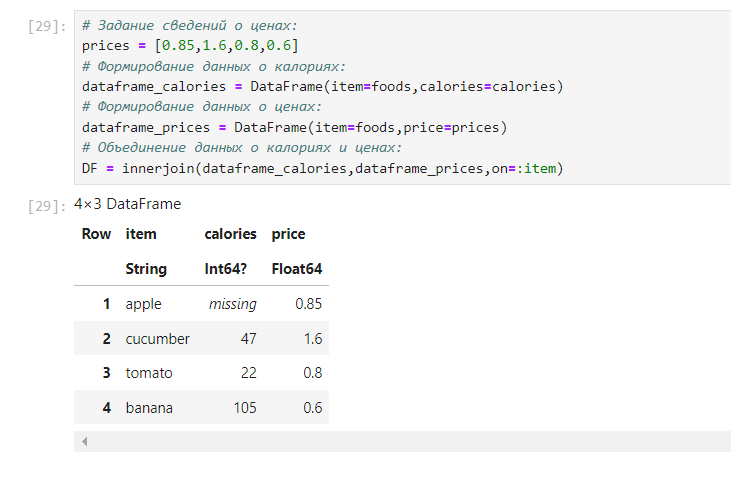
\includegraphics[width=0.8\linewidth,height=0.8\textheight]{image/21.PNG}

}

\caption{Формирование таблиц данных и их объединение в один фрейм}

\end{figure}%
\end{frame}

\begin{frame}{2.23 FileIO}
\phantomsection\label{fileio}
\begin{figure}

{\centering 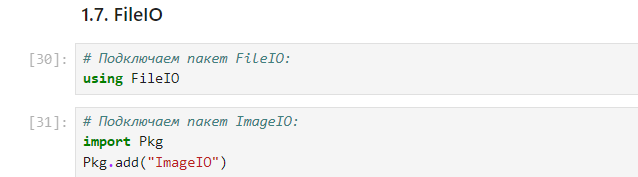
\includegraphics[width=1\linewidth,height=1\textheight]{image/22.PNG}

}

\caption{Подключение пакетов}

\end{figure}%
\end{frame}

\begin{frame}{2.24 FileIO}
\phantomsection\label{fileio-1}
\begin{figure}

{\centering 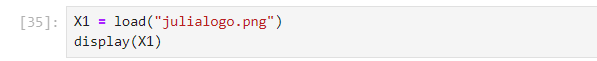
\includegraphics[width=1\linewidth,height=1\textheight]{image/23.PNG}

}

\caption{Загрузка изображения}

\end{figure}%
\end{frame}

\begin{frame}{2.25 FileIO}
\phantomsection\label{fileio-2}
\begin{figure}

{\centering 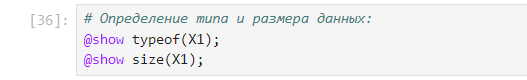
\includegraphics[width=1\linewidth,height=1\textheight]{image/24.PNG}

}

\caption{Определение типа и размера данных}

\end{figure}%
\end{frame}

\begin{frame}{2.26 Обработка данных: стандартные алгоритмы машинного
обучения в Julia. Кластеризация данных. Метод k-средних}
\phantomsection\label{ux43eux431ux440ux430ux431ux43eux442ux43aux430-ux434ux430ux43dux43dux44bux445-ux441ux442ux430ux43dux434ux430ux440ux442ux43dux44bux435-ux430ux43bux433ux43eux440ux438ux442ux43cux44b-ux43cux430ux448ux438ux43dux43dux43eux433ux43e-ux43eux431ux443ux447ux435ux43dux438ux44f-ux432-julia.-ux43aux43bux430ux441ux442ux435ux440ux438ux437ux430ux446ux438ux44f-ux434ux430ux43dux43dux44bux445.-ux43cux435ux442ux43eux434-k-ux441ux440ux435ux434ux43dux438ux445}
\begin{figure}

{\centering 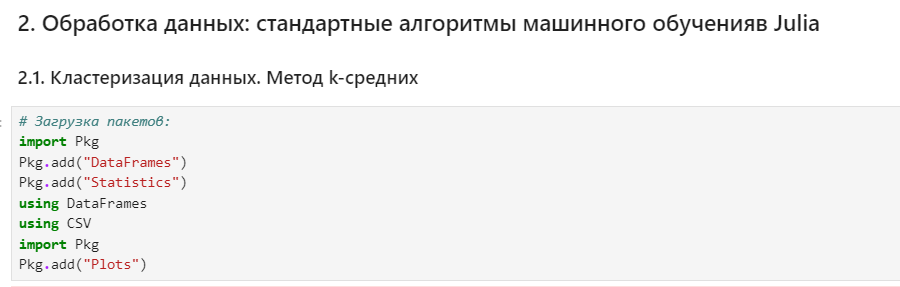
\includegraphics[width=1\linewidth,height=1\textheight]{image/25.PNG}

}

\caption{Подключение нужных пакетов}

\end{figure}%
\end{frame}

\begin{frame}{2.27 Обработка данных: стандартные алгоритмы машинного
обучения в Julia. Кластеризация данных. Метод k-средних}
\phantomsection\label{ux43eux431ux440ux430ux431ux43eux442ux43aux430-ux434ux430ux43dux43dux44bux445-ux441ux442ux430ux43dux434ux430ux440ux442ux43dux44bux435-ux430ux43bux433ux43eux440ux438ux442ux43cux44b-ux43cux430ux448ux438ux43dux43dux43eux433ux43e-ux43eux431ux443ux447ux435ux43dux438ux44f-ux432-julia.-ux43aux43bux430ux441ux442ux435ux440ux438ux437ux430ux446ux438ux44f-ux434ux430ux43dux43dux44bux445.-ux43cux435ux442ux43eux434-k-ux441ux440ux435ux434ux43dux438ux445-1}
\begin{figure}

{\centering 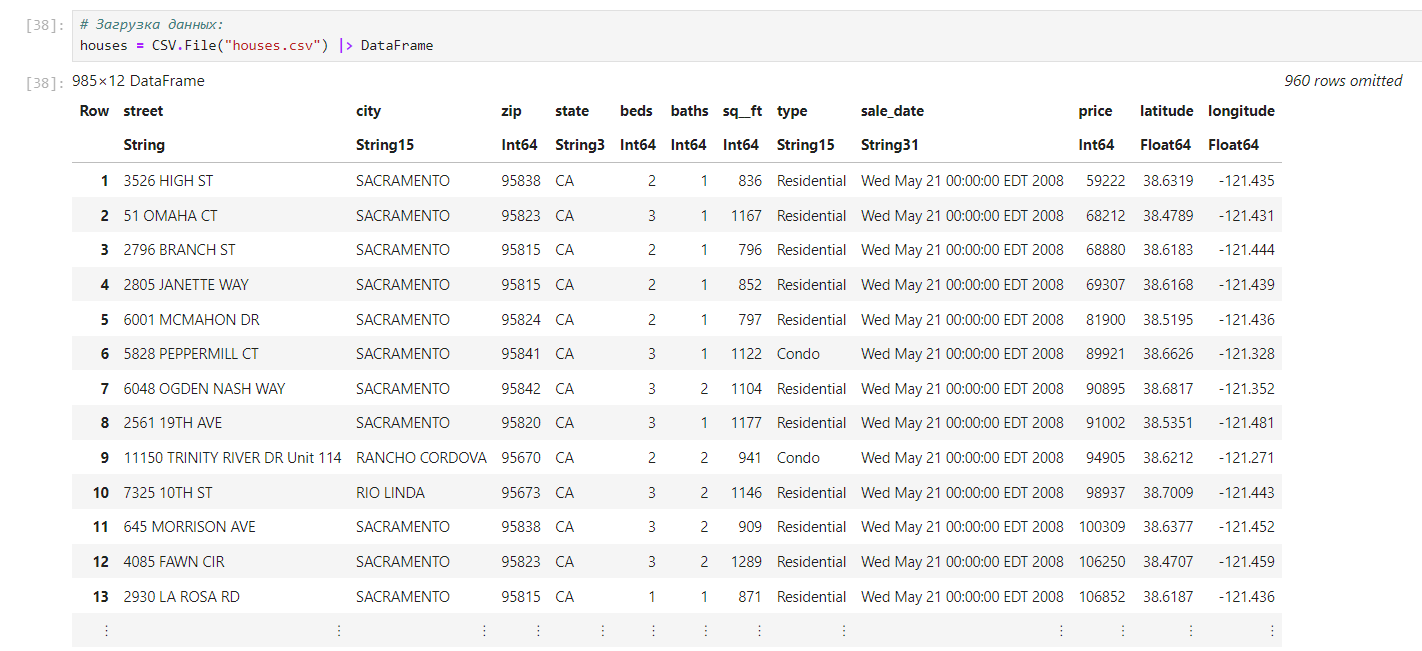
\includegraphics[width=0.8\linewidth,height=0.8\textheight]{image/26.PNG}

}

\caption{Загрузка данных}

\end{figure}%
\end{frame}

\begin{frame}{2.28 Обработка данных: стандартные алгоритмы машинного
обучения в Julia. Кластеризация данных. Метод k-средних}
\phantomsection\label{ux43eux431ux440ux430ux431ux43eux442ux43aux430-ux434ux430ux43dux43dux44bux445-ux441ux442ux430ux43dux434ux430ux440ux442ux43dux44bux435-ux430ux43bux433ux43eux440ux438ux442ux43cux44b-ux43cux430ux448ux438ux43dux43dux43eux433ux43e-ux43eux431ux443ux447ux435ux43dux438ux44f-ux432-julia.-ux43aux43bux430ux441ux442ux435ux440ux438ux437ux430ux446ux438ux44f-ux434ux430ux43dux43dux44bux445.-ux43cux435ux442ux43eux434-k-ux441ux440ux435ux434ux43dux438ux445-2}
\begin{figure}

{\centering 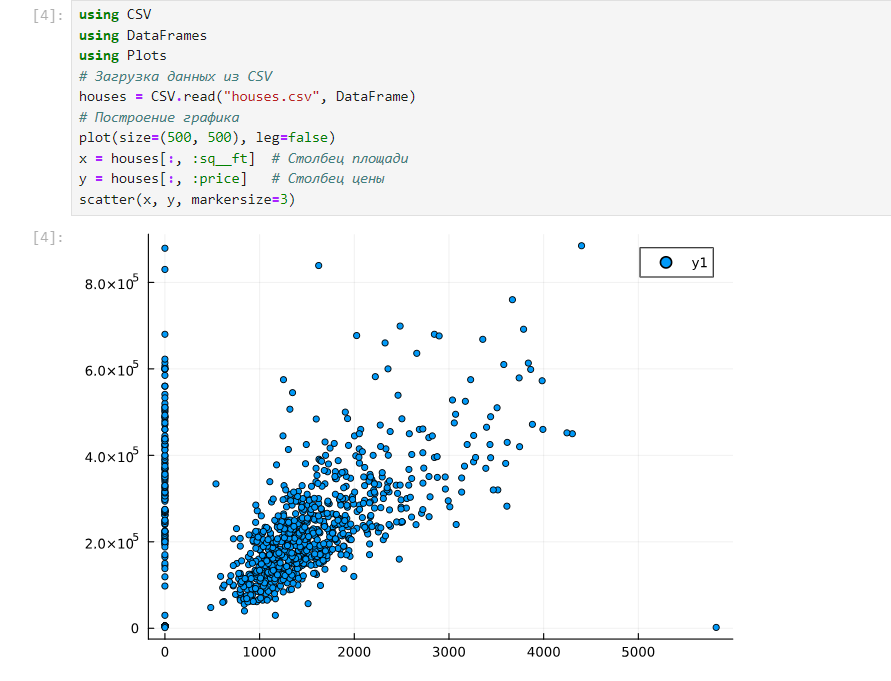
\includegraphics[width=0.8\linewidth,height=0.8\textheight]{image/27.PNG}

}

\caption{Построение графика цен на недвижимость в зависимости от
площади}

\end{figure}%
\end{frame}

\begin{frame}{2.29 Обработка данных: стандартные алгоритмы машинного
обучения в Julia. Кластеризация данных. Метод k-средних}
\phantomsection\label{ux43eux431ux440ux430ux431ux43eux442ux43aux430-ux434ux430ux43dux43dux44bux445-ux441ux442ux430ux43dux434ux430ux440ux442ux43dux44bux435-ux430ux43bux433ux43eux440ux438ux442ux43cux44b-ux43cux430ux448ux438ux43dux43dux43eux433ux43e-ux43eux431ux443ux447ux435ux43dux438ux44f-ux432-julia.-ux43aux43bux430ux441ux442ux435ux440ux438ux437ux430ux446ux438ux44f-ux434ux430ux43dux43dux44bux445.-ux43cux435ux442ux43eux434-k-ux441ux440ux435ux434ux43dux438ux445-3}
\begin{figure}

{\centering 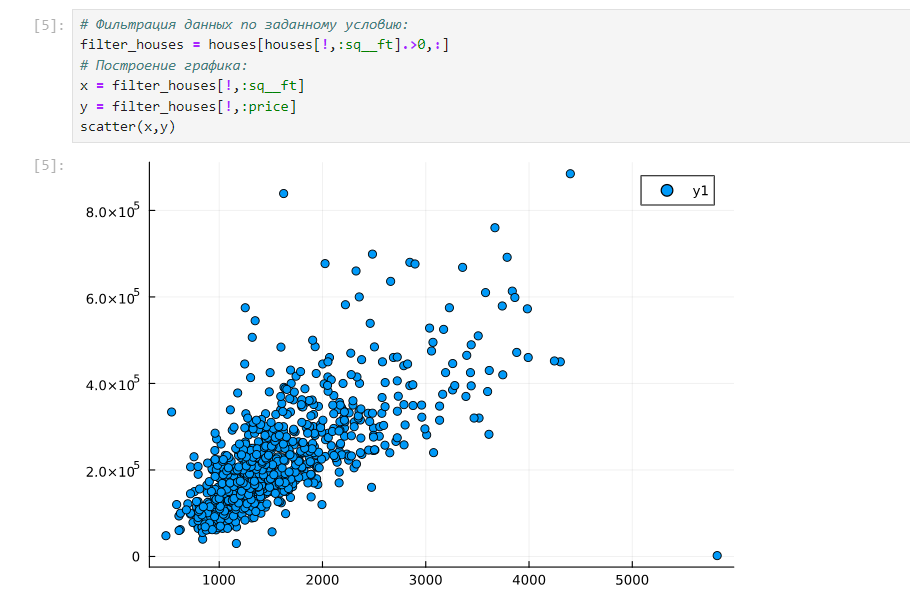
\includegraphics[width=0.8\linewidth,height=0.8\textheight]{image/28.PNG}

}

\caption{Построение графика без \enquote{артефактов}}

\end{figure}%
\end{frame}

\begin{frame}{2.30 Обработка данных: стандартные алгоритмы машинного
обучения в Julia. Кластеризация данных. Метод k-средних}
\phantomsection\label{ux43eux431ux440ux430ux431ux43eux442ux43aux430-ux434ux430ux43dux43dux44bux445-ux441ux442ux430ux43dux434ux430ux440ux442ux43dux44bux435-ux430ux43bux433ux43eux440ux438ux442ux43cux44b-ux43cux430ux448ux438ux43dux43dux43eux433ux43e-ux43eux431ux443ux447ux435ux43dux438ux44f-ux432-julia.-ux43aux43bux430ux441ux442ux435ux440ux438ux437ux430ux446ux438ux44f-ux434ux430ux43dux43dux44bux445.-ux43cux435ux442ux43eux434-k-ux441ux440ux435ux434ux43dux438ux445-4}
\begin{figure}

{\centering 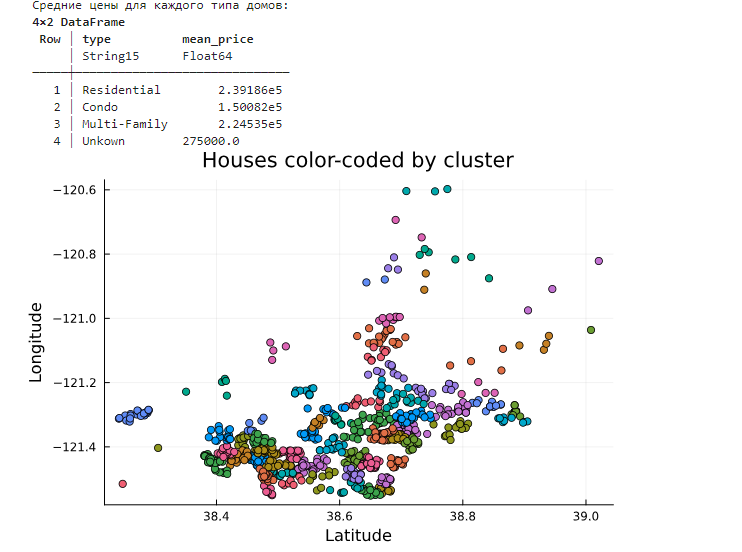
\includegraphics[width=0.8\linewidth,height=0.8\textheight]{image/29.PNG}

}

\caption{Построение графика с кластерами разных цветов}

\end{figure}%
\end{frame}

\begin{frame}{2.31 Обработка данных: стандартные алгоритмы машинного
обучения в Julia. Кластеризация данных. Метод k-средних}
\phantomsection\label{ux43eux431ux440ux430ux431ux43eux442ux43aux430-ux434ux430ux43dux43dux44bux445-ux441ux442ux430ux43dux434ux430ux440ux442ux43dux44bux435-ux430ux43bux433ux43eux440ux438ux442ux43cux44b-ux43cux430ux448ux438ux43dux43dux43eux433ux43e-ux43eux431ux443ux447ux435ux43dux438ux44f-ux432-julia.-ux43aux43bux430ux441ux442ux435ux440ux438ux437ux430ux446ux438ux44f-ux434ux430ux43dux43dux44bux445.-ux43cux435ux442ux43eux434-k-ux441ux440ux435ux434ux43dux438ux445-5}
\begin{figure}

{\centering 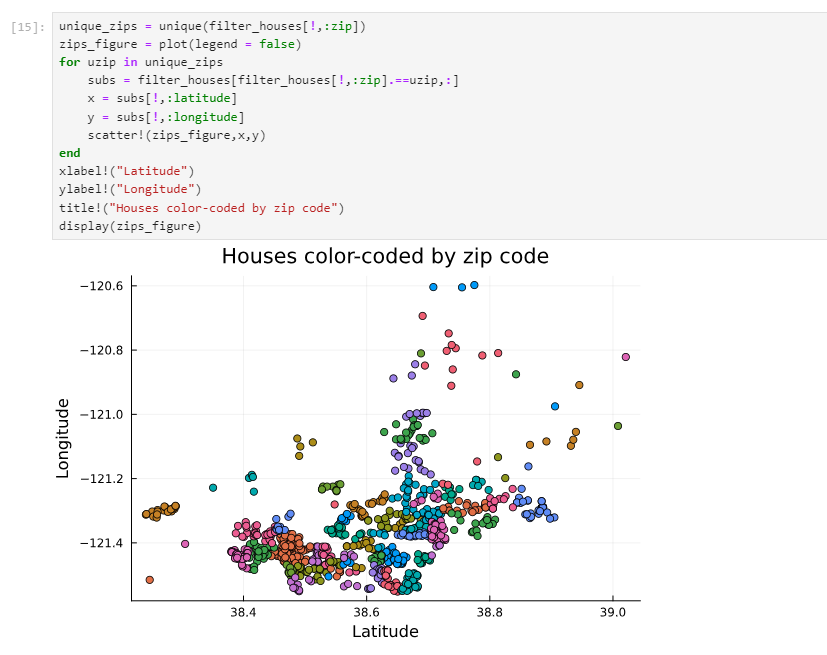
\includegraphics[width=0.8\linewidth,height=0.8\textheight]{image/30.PNG}

}

\caption{Построение графика с кластерами разных цветов по почтовому
индексу}

\end{figure}%
\end{frame}

\begin{frame}{2.32 Кластеризация данных. Метод k ближайших соседей}
\phantomsection\label{ux43aux43bux430ux441ux442ux435ux440ux438ux437ux430ux446ux438ux44f-ux434ux430ux43dux43dux44bux445.-ux43cux435ux442ux43eux434-k-ux431ux43bux438ux436ux430ux439ux448ux438ux445-ux441ux43eux441ux435ux434ux435ux439}
\begin{figure}

{\centering 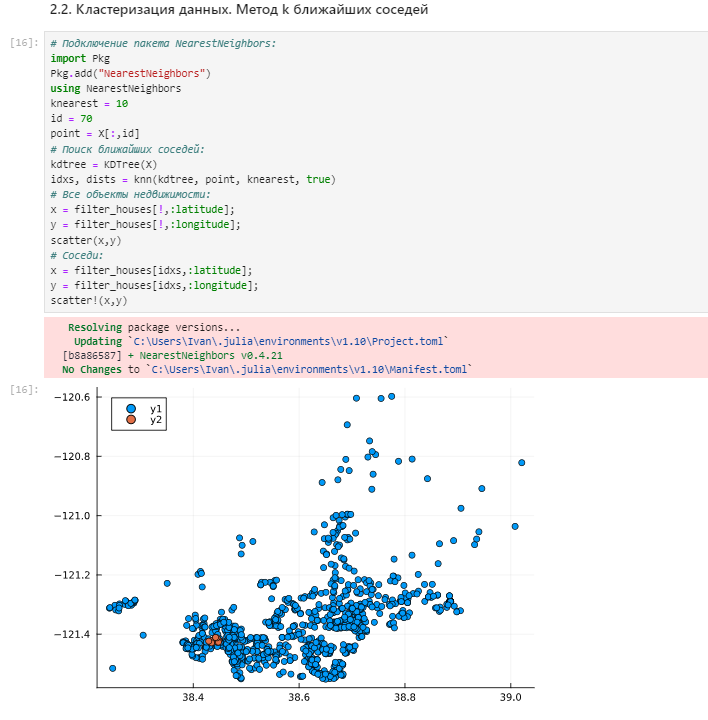
\includegraphics[width=0.8\linewidth,height=0.8\textheight]{image/31.PNG}

}

\caption{Отображение на графике соседей выбранного объекта недвижимости}

\end{figure}%
\end{frame}

\begin{frame}{2.33 Кластеризация данных. Метод k ближайших соседей}
\phantomsection\label{ux43aux43bux430ux441ux442ux435ux440ux438ux437ux430ux446ux438ux44f-ux434ux430ux43dux43dux44bux445.-ux43cux435ux442ux43eux434-k-ux431ux43bux438ux436ux430ux439ux448ux438ux445-ux441ux43eux441ux435ux434ux435ux439-1}
\begin{figure}

{\centering 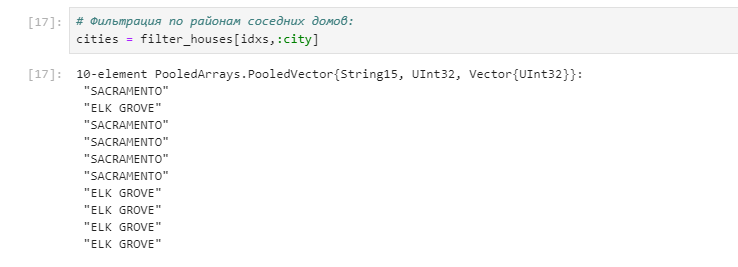
\includegraphics[width=1\linewidth,height=1\textheight]{image/32.PNG}

}

\caption{Определение районов соседних домов}

\end{figure}%
\end{frame}

\begin{frame}{2.34 Обработка данных. Метод главных компонент}
\phantomsection\label{ux43eux431ux440ux430ux431ux43eux442ux43aux430-ux434ux430ux43dux43dux44bux445.-ux43cux435ux442ux43eux434-ux433ux43bux430ux432ux43dux44bux445-ux43aux43eux43cux43fux43eux43dux435ux43dux442}
\begin{figure}

{\centering 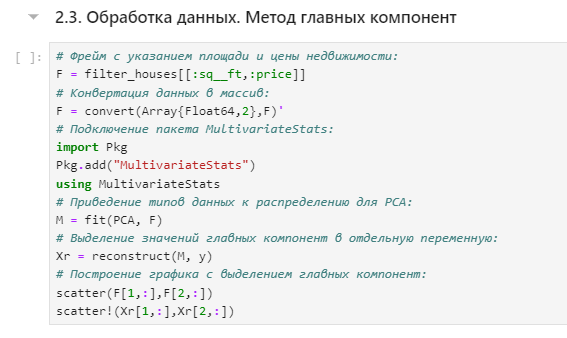
\includegraphics[width=0.8\linewidth,height=0.8\textheight]{image/33.PNG}

}

\caption{Попытка уменьшения размера данных о цене и площади из набора
данных домов}

\end{figure}%
\end{frame}

\begin{frame}{2.35 Обработка данных. Линейная регрессия}
\phantomsection\label{ux43eux431ux440ux430ux431ux43eux442ux43aux430-ux434ux430ux43dux43dux44bux445.-ux43bux438ux43dux435ux439ux43dux430ux44f-ux440ux435ux433ux440ux435ux441ux441ux438ux44f}
\begin{figure}

{\centering 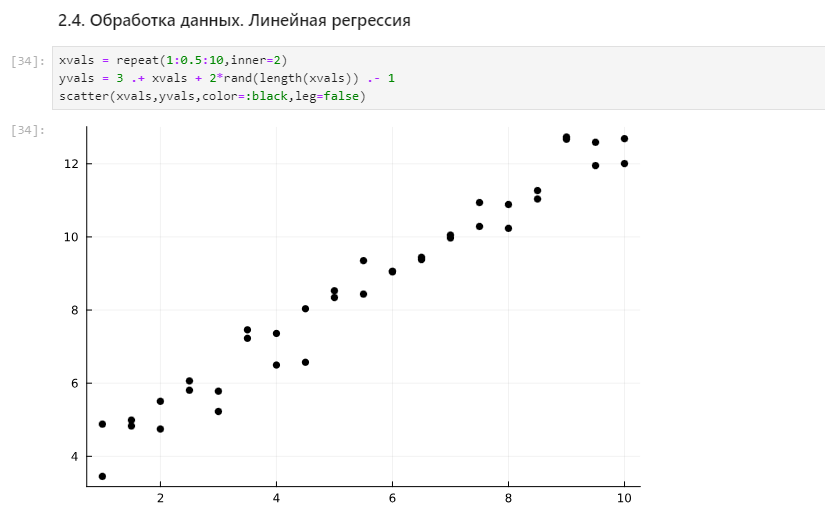
\includegraphics[width=0.8\linewidth,height=0.8\textheight]{image/34.PNG}

}

\caption{Исходные данные}

\end{figure}%
\end{frame}

\begin{frame}{2.36 Обработка данных. Линейная регрессия}
\phantomsection\label{ux43eux431ux440ux430ux431ux43eux442ux43aux430-ux434ux430ux43dux43dux44bux445.-ux43bux438ux43dux435ux439ux43dux430ux44f-ux440ux435ux433ux440ux435ux441ux441ux438ux44f-1}
\begin{figure}

{\centering 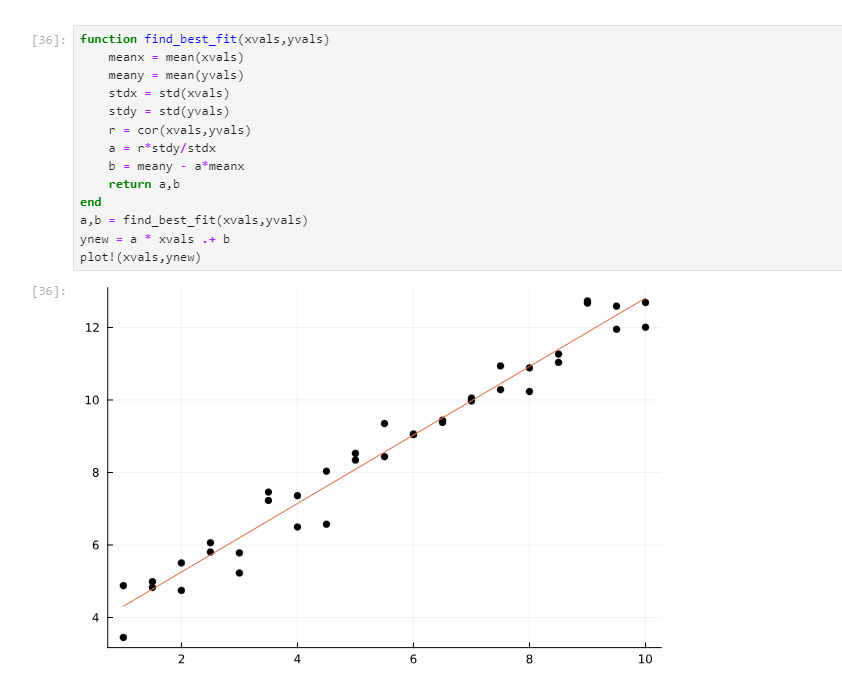
\includegraphics[width=0.8\linewidth,height=0.8\textheight]{image/35.PNG}

}

\caption{Применение функции для построения графика}

\end{figure}%
\end{frame}

\begin{frame}{2.37 Обработка данных. Линейная регрессия}
\phantomsection\label{ux43eux431ux440ux430ux431ux43eux442ux43aux430-ux434ux430ux43dux43dux44bux445.-ux43bux438ux43dux435ux439ux43dux430ux44f-ux440ux435ux433ux440ux435ux441ux441ux438ux44f-2}
\begin{figure}

{\centering 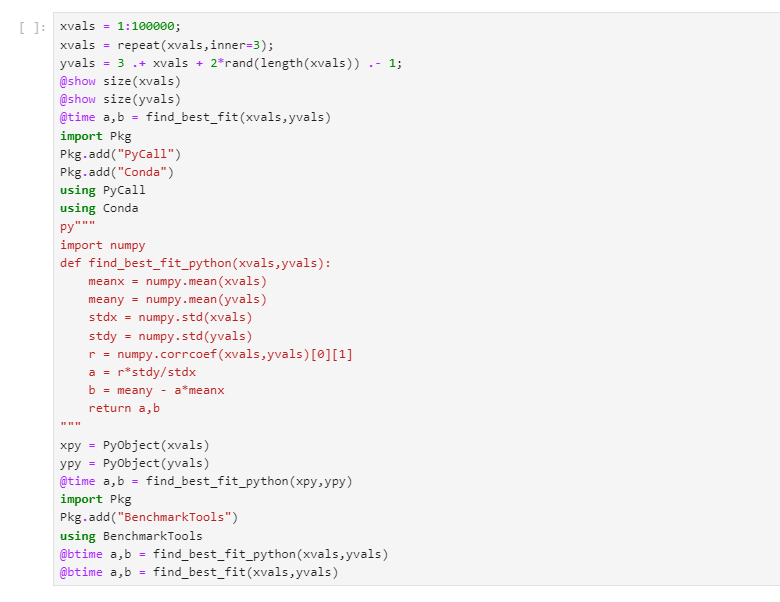
\includegraphics[width=0.8\linewidth,height=0.8\textheight]{image/36.PNG}

}

\caption{Сравнение}

\end{figure}%
\end{frame}

\begin{frame}{2.38 Самостоятельная работа}
\phantomsection\label{ux441ux430ux43cux43eux441ux442ux43eux44fux442ux435ux43bux44cux43dux430ux44f-ux440ux430ux431ux43eux442ux430}
\begin{figure}

{\centering 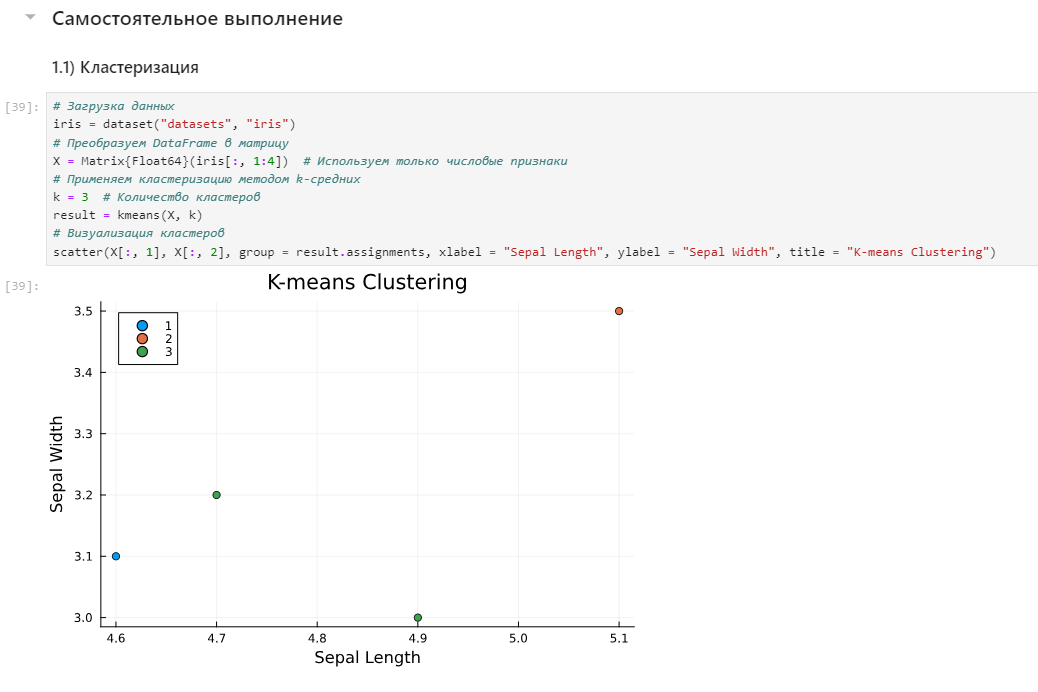
\includegraphics[width=0.8\linewidth,height=0.8\textheight]{image/37.PNG}

}

\caption{Решение задания №1}

\end{figure}%
\end{frame}

\begin{frame}{2.39 Самостоятельная работа}
\phantomsection\label{ux441ux430ux43cux43eux441ux442ux43eux44fux442ux435ux43bux44cux43dux430ux44f-ux440ux430ux431ux43eux442ux430-1}
\begin{figure}

{\centering 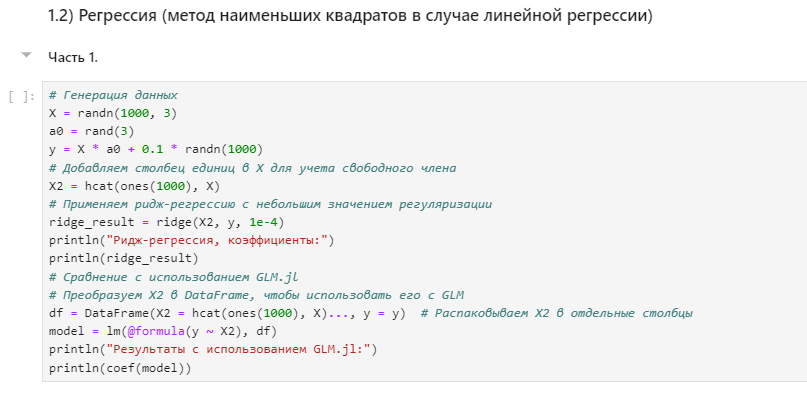
\includegraphics[width=0.8\linewidth,height=0.8\textheight]{image/38.PNG}

}

\caption{Решение задания №2}

\end{figure}%
\end{frame}

\begin{frame}{2.40 Самостоятельная работа}
\phantomsection\label{ux441ux430ux43cux43eux441ux442ux43eux44fux442ux435ux43bux44cux43dux430ux44f-ux440ux430ux431ux43eux442ux430-2}
\begin{figure}

{\centering 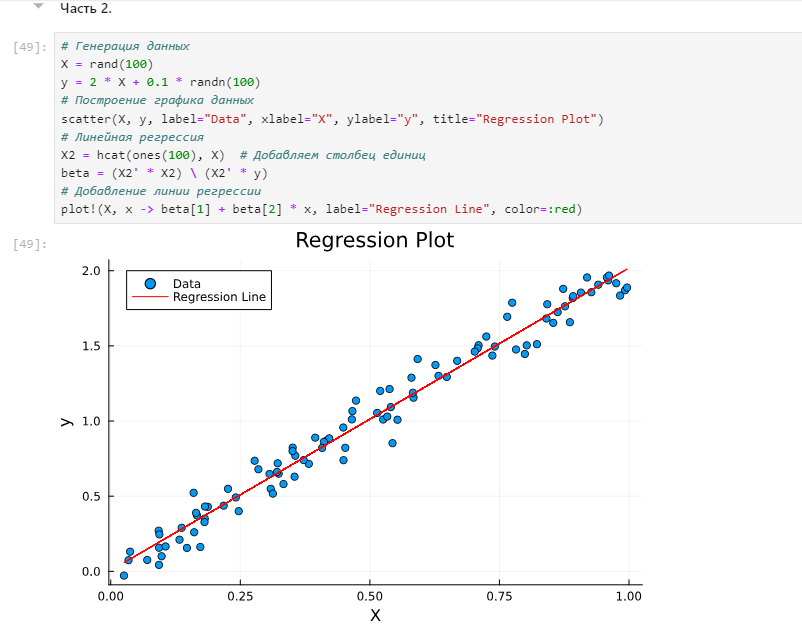
\includegraphics[width=0.8\linewidth,height=0.8\textheight]{image/39.PNG}

}

\caption{Решение задания №2}

\end{figure}%
\end{frame}

\begin{frame}{2.41 Самостоятельная работа}
\phantomsection\label{ux441ux430ux43cux43eux441ux442ux43eux44fux442ux435ux43bux44cux43dux430ux44f-ux440ux430ux431ux43eux442ux430-3}
\begin{figure}

{\centering 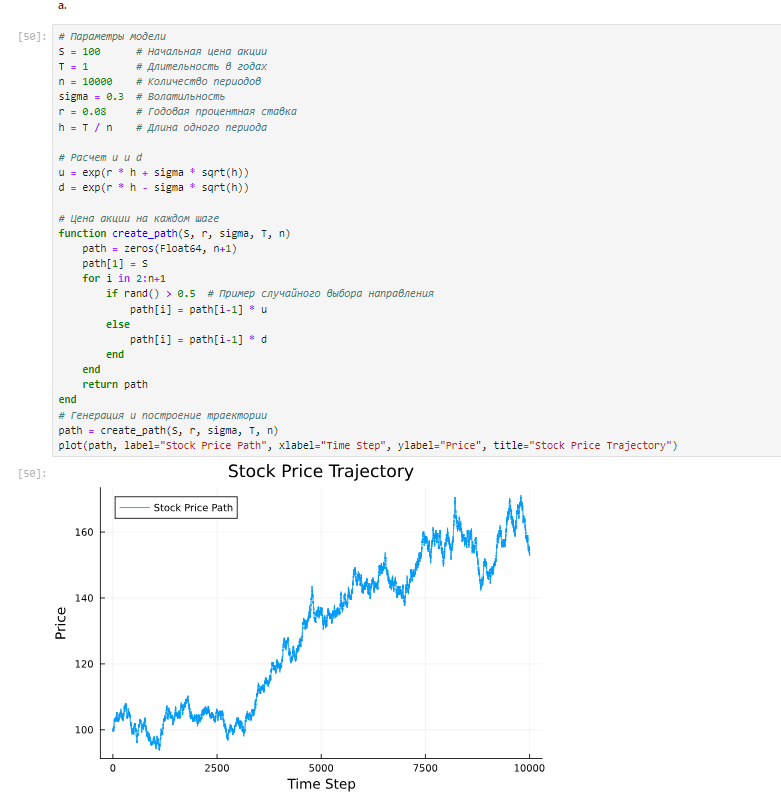
\includegraphics[width=0.8\linewidth,height=0.8\textheight]{image/40.PNG}

}

\caption{Решение задания №3}

\end{figure}%
\end{frame}

\begin{frame}{2.42 Самостоятельная работа}
\phantomsection\label{ux441ux430ux43cux43eux441ux442ux43eux44fux442ux435ux43bux44cux43dux430ux44f-ux440ux430ux431ux43eux442ux430-4}
\begin{figure}

{\centering 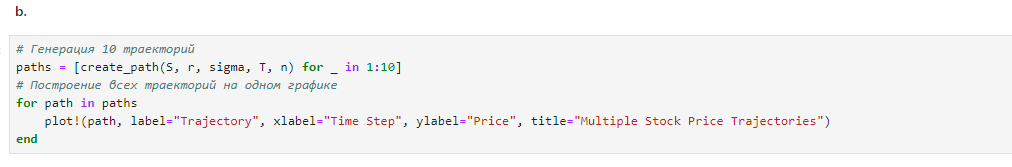
\includegraphics[width=1\linewidth,height=1\textheight]{image/41.PNG}

}

\caption{Решение задания №3}

\end{figure}%
\end{frame}

\begin{frame}{2.43 Самостоятельная работа}
\phantomsection\label{ux441ux430ux43cux43eux441ux442ux43eux44fux442ux435ux43bux44cux43dux430ux44f-ux440ux430ux431ux43eux442ux430-5}
\begin{figure}

{\centering 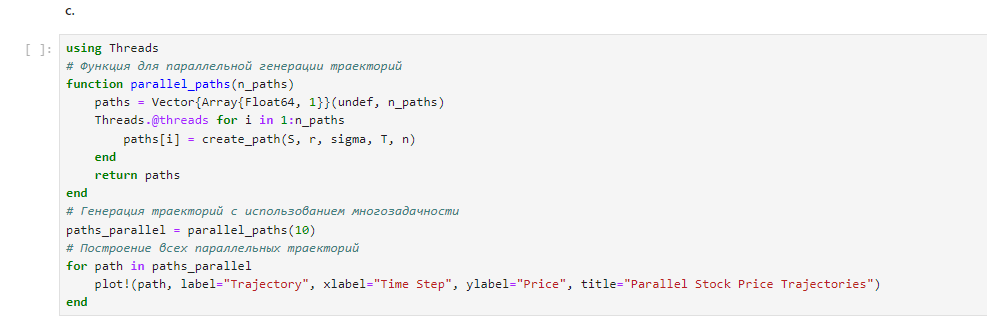
\includegraphics[width=1\linewidth,height=1\textheight]{image/42.PNG}

}

\caption{Решение задания №3}

\end{figure}%
\end{frame}

\section{3. Вывод}\label{ux432ux44bux432ux43eux434}

\begin{frame}{3.1 Вывод}
\phantomsection\label{ux432ux44bux432ux43eux434-1}
\begin{itemize}[<+->]
\tightlist
\item
  В ходе выполнения лабораторной работы были изучены специализированные
  пакеты Julia для обработки данных.
\end{itemize}
\end{frame}
\end{column}
\end{columns}
\end{frame}




\end{document}
